\documentclass[article]{jss}
\usepackage[utf8]{inputenc}

\providecommand{\tightlist}{%
  \setlength{\itemsep}{0pt}\setlength{\parskip}{0pt}}

\author{
Anna Michalek\\European Central Bank \And Alain Quartier-La-Tente\\Insee
}
\title{\pkg{RJDemetra}: A R Interface To JDemetra+ Seasonal Adjustment Software}

\Plainauthor{Anna Michalek, Alain Quartier-La-Tente}
\Plaintitle{A Capitalized Title: Something about a Package foo}
\Shorttitle{\pkg{RJDemetra}: A R Interface To JDemetra+ Seasonal Adjustment Software}

\Abstract{
The abstract of the article.
}

\Keywords{\proglang{R}, seasonal adjustment, time series}
\Plainkeywords{R, seasonal adjustment, time series}

%% publication information
%% \Volume{50}
%% \Issue{9}
%% \Month{June}
%% \Year{2012}
%% \Submitdate{}
%% \Acceptdate{2012-06-04}

\Address{
    }

% Pandoc header

\usepackage{amsmath} \usepackage{booktabs} \usepackage{longtable} \usepackage{array} \usepackage{multirow} \usepackage{wrapfig} \usepackage{float} \usepackage{pdflscape} \usepackage{tabu} \usepackage{threeparttable} \usepackage{threeparttablex} \usepackage[normalem]{ulem} \usepackage{makecell}

\begin{document}

\hypertarget{introduction}{%
\section{Introduction}\label{introduction}}

The package \pkg{RJDemetra} provides a R interface to the seasonal
adjustment software JDemetra+. Note that, JDemetra+ being implemented in
Java, \pkg{RJDemetra} relies on the \pkg{rJava} package and Java SE 8 or
later version is required. The two leading seasonal adjustment methods
TRAMO/SEATS+ and X-12ARIMA/X-13ARIMA-SEATS can be used with all the
specifications defined in JDemetra+.

This article is structured as following. In the first section the .. is
presented.

\hypertarget{seasonal-adjustment-in-brief}{%
\subsection{Seasonal adjustment in
brief}\label{seasonal-adjustment-in-brief}}

The \textbf{first step} of seasonal adjustment, both in
X-12ARIMA/X-13ARIMA-SEATS and TRAMO-SEATS+, consists of pre-adjusting
the time series by removing from it the deterministic effects and
estimating missing observations. Among deterministic effects, we
distinguish outliers, calendar and regression effects. In this step,
also forecasts and backcasts of the pre-adjusted series are estimated
which allows applying linear filters at both ends of the series in the
second step of the seasonal adjustment. The pre-adjustment,
linearization, of the input series is achieved with a \textbf{RegARIMA}
model (model with ARIMA errors) as specified below.

\[z_t=y_t\beta+x_t\] where

\begin{itemize}
\tightlist
\item
  \(z_t\) - is the original series;
\item
  \(\beta = (\beta_1,...,\beta_n)\) - a vector of regression
  coefficients;
\item
  \(y_t = (y_{1t},...,y_{nt})\) - \(n\) regression variables (outliers,
  calendar effects, user-defined variables);
\item
  \(x_t\) - a disturbance that follows the general ARIMA process:
\item
  \(\phi(B)\delta(B)x_t=\theta(B)a_t\); \(\phi(B), \delta(B)\) and
  \(\theta(B)\) are the finite polynomials in \(B\); \(a_t\) is a
  white-noise variable with zero mean and a constant variance.
\end{itemize}

The polynomial \(\phi(B)\) is a stationary autoregressive (AR)
polynomial in \(B\), which is a product of the stationary regular AR
polynomial in \(B\) and the stationary seasonal polynomial in \(B^s\):

\[\phi(B)=\phi_p(B)\Phi_{bp}(B^s)=(1+\phi_1B+...+\phi_pB^p)(1+\Phi_1B^s+...+\Phi_{bp}B^{bps}\]

where:

\begin{itemize}
\tightlist
\item
  \(p\) - number of regular AR terms (in the package and in JDemetra+
  \(p \le 3\));
\item
  \(bp\) - number of seasonal AR terms (in the package and in JDemetra+
  \(bp \le 1\));
\item
  \(s\) - number of observations per year (frequency of the time
  series).
\end{itemize}

The polynomial \(\theta(B)\) is an invertible moving average (MA)
polynomial in \(B\), which is a product of the invertible regular MA
polynomial in \(B\) and the invertible seasonal MA polynomial in
\(B^s\):

\[\theta(B)=\theta_q(B)\Theta_{bq}(B^s)=(1+\theta_1B+...+\theta_qB^q)(1+\Theta_1B^s+...+\Theta_{bq}B^{bqs})\]

where:

\begin{itemize}
\tightlist
\item
  \(q\) - number of regular MA terms (in the package and in JDemetra+
  \(q \le 3\));
\item
  \(bq\) - number of seasonal MA terms (in the package and in JDemetra+
  \(bq \le 1\));
\end{itemize}

The polynomial \(\delta(B)\) is the non-stationary AR polynomial in
\(B\) (unit roots):

\[\delta(B)=(1-B)^d(1-B^s)^{d_s}\]

where:

\begin{itemize}
\tightlist
\item
  \(d\) - regular differencing order (in the package and in JDemetra+
  \(d \le 1\));
\item
  \(d_s\) - seasonal differencing order (in the package and in JDemetra+
  \(d_s \le 1\));
\end{itemize}

In the \textbf{second part} of seasonal adjustment, called the
\textbf{decomposition}, the pre-adjusted series is decomposed into the
following components: trend-cycle (\code{t}), seasonal component
(\code{s}) and irregular component (\code{i}). The decomposition can be:

\begin{itemize}
\tightlist
\item
  additive (\code{y = t + s + i})
\item
  multiplicative (\code{y = t * s * i})
\item
  log-additive (\code{log(y) = log(t)+log(s)+log(i)}) or
\item
  pseudo-additive (\code{y = t*(s+i-1)})
\end{itemize}

The last two decompositions are available only under X13.

The method of decomposing the pre-adjusted series differs between
TRAMO-SEATS+ and X-12ARIMA/X-13ARIMA. In TRAMO-SEATS+, SEATS (``Signal
Extraction in ARIMA Time Series'') decomposes the observed series with a
ARIMA-model based method. Whereas in X-12ARIMA/X-13ARIMA, the X11
algorithm decomposes the time series by means of linear filters. More
information on the TRAMO-SEATS+ method can be found on the Bank of Spain
website (\href{www.bde.es}{link}) and on X-12ARIMA/X-13ARIMA, on the
U.S. Census Bureau website.

As a result of seasonal adjustment, the final seasonally adjusted series
(\code{sa}) shall be free of seasonal and calendar-related movements.

More details on the methodlogy used in JDemetra+ can be found in the
JDemetra+ manuals and user guides available at
\href{https://ec.europa.eu/eurostat/cros/content/documentation_en}{link}.

\hypertarget{rjdemetra-basics}{%
\section{RJDemetra basics}\label{rjdemetra-basics}}

The \pkg{RJDemetra} package alows to:

\begin{itemize}
\tightlist
\item
  create and modify model specifications
\item
  create and modify models
\item
  import/export JDemetra+ workspaces
\end{itemize}

\hypertarget{dataset}{%
\subsection{Dataset}\label{dataset}}

In this package the sts\_inpr\_m database of Eurostat is included, which
contains monthly industrial production indices in manufacturing in the
European Union. It contains 37 time series from january 1990 to december
2017 which are considered to be affected by seasonal and working day
effects. The data is a \code{ts} object and can be accessed using the
\code{ipi_c_eu} object. The following snippet of code plots the
industrial production index of the euro aera (EA19):

\begin{CodeChunk}

\begin{CodeInput}
R> library(RJDemetra)
R> plot(ipi_c_eu[, "EA19"])
\end{CodeInput}


\begin{center}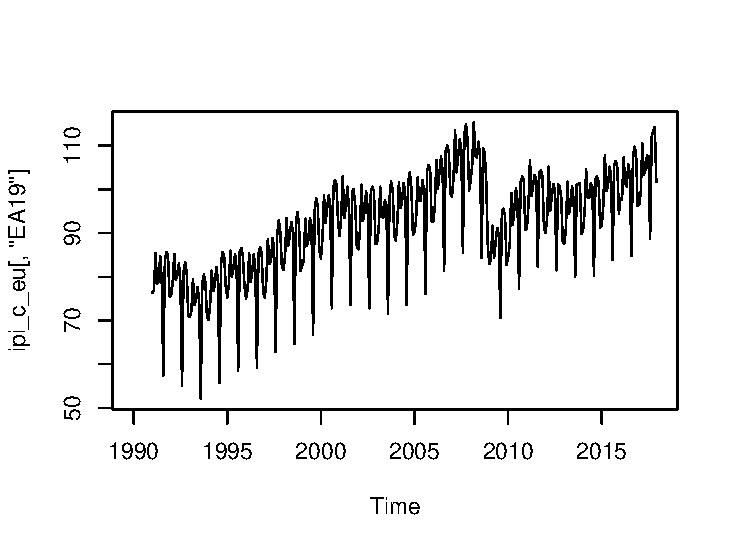
\includegraphics{img/img-basic_raw_data_plot-1} \end{center}

\end{CodeChunk}

\hypertarget{estimate-a-pre-defined-regarima-and-sa-model}{%
\section{Estimate a pre-defined RegARIMA and SA
model}\label{estimate-a-pre-defined-regarima-and-sa-model}}

As in JDemetra+, the \pkg{RJDemetra} package allows to perform seasonal
adjustment using pre-defined model specifications. The specifications
are separately defined for TRAMO-SEATS and X-13ARIMA-SEATS estimation
methods. It is also possible to perform only the first step of seasonal
adjustment; the RegARIMA estimation. The pre-defined model
specifications are described in tables \ref{tab:pre_def_ts} and
\ref{tab:pre_def_x13}. They are identical for pre-adjustment (column 1)
and for seasonal adjustment (column 2). The pre-defined specifications
correspond to most commonly used specifications and users are
recommended to start their analysis with one of them. In section 5 it is
presented how to modify model specifications, including the possibility
to incorprate user-defined regressors.

\begin{table}[t]

\caption{\label{tab:pre_def_ts}Pre-defined specification for TRAMO and TRAMO-SEATS}
\centering
\fontsize{7}{9}\selectfont
\begin{tabular}{c>{\centering\arraybackslash}p{1.cm}>{\centering\arraybackslash}p{1.cm}>{\centering\arraybackslash}p{1.5cm}>{\centering\arraybackslash}p{0.9cm}>{\centering\arraybackslash}p{0.9cm}>{\centering\arraybackslash}p{1.5cm}>{\centering\arraybackslash}p{0.9cm}c}
\toprule
\multicolumn{2}{c}{Specification} & \multicolumn{1}{c}{} \\
\cmidrule(l{3pt}r{3pt}){1-2}
TRAMO & TRAMO-SEATS & Trans-formation & Pre-adjust-ment for leap-year & Working days & Trading days & Easter effect & Outliers & ARIMA model\\
\midrule
TR0 & RSA0 & no & no & no & no & no & no & (0,1,1)(0,1,1)\\
TR1 & RSA1 & test & no & no & no & no & test & (0,1,1)(0,1,1)\\
TR2 & RSA2 & test & no & test & no & test & test & (0,1,1)(0,1,1)\\
TR3 & RSA3 & test & no & no & no & no & test & AMI\\
TR4 & RSA4 & test & no & test & no & test & test & AMI\\
\addlinespace
TR5 & RSA5 & test & no & no & yes & test (Standard) & test & AMI\\
TRfull (default) & RSAfull (default) & test & yes & no & test & test (Include Easter) & test & AMI\\
\bottomrule
\end{tabular}
\end{table}

\begin{table}[t]

\caption{\label{tab:pre_def_x13}Pre-defined specification for RegARIMA and X-13ARIMA-SEATS}
\centering
\fontsize{7}{9}\selectfont
\begin{tabular}{c>{\centering\arraybackslash}p{1.7cm}>{\centering\arraybackslash}p{1.cm}>{\centering\arraybackslash}p{1.4cm}>{\centering\arraybackslash}p{0.9cm}>{\centering\arraybackslash}p{0.9cm}>{\centering\arraybackslash}p{0.9cm}>{\centering\arraybackslash}p{0.9cm}c}
\toprule
\multicolumn{2}{c}{Specification} & \multicolumn{1}{c}{} \\
\cmidrule(l{3pt}r{3pt}){1-2}
RegARIMA & X-13ARIMA-SEATS & Trans-formation & Pre-adjust-ment for leap-year & Working days & Trading days & Easter effect & Outliers & ARIMA model\\
\midrule
RG0 & X11 & no & no & no & no & no & no & (0,1,1)(0,1,1)\\
RG1 & RSA1 & test & no & no & no & no & test & (0,1,1)(0,1,1)\\
RG2c & RSA2c & test & test & test & no & test & test & (0,1,1)(0,1,1)\\
RG3 & RSA3 & test & no & no & no & no & test & AMI\\
RG4c & RSA4c & test & test & test & no & test & test & AMI\\
\addlinespace
RG5c (default) & RSA5 (default) & test & test & no & test & test & test & AMI\\
\bottomrule
\end{tabular}
\end{table}

The below code presents how to perform an estimation, with pre-defined
specifications, of:

\begin{itemize}
\tightlist
\item
  RegARIMA

  \begin{itemize}
  \tightlist
  \item
    X-13ARIMA method:
    \code{regarima_def_x13(series, spec = c("RG5c", "RG0", "RG1", "RG2c", "RG3","RG4c"))}
  \item
    TRAMO-SEATS method:
    \code{regarima_def_tramoseats(series, spec = c("TRfull", "TR0","TR1", "TR2","TR3", "TR4","TR5"))}
  \end{itemize}
\item
  Seasonal adjustment

  \begin{itemize}
  \tightlist
  \item
    X-13ARIMA method:
    \code{x13_def(series, spec = c("RSA5c", "RSA0", "RSA1", "RSA2c", "RSA3","RSA4c"), userdefined = NULL)}
  \item
    TRAMO-SEATS method:
    \code{tramoseats_def(series, spec = c("RSAfull", "RSA0", "RSA1", "RSA2", "RSA", "RSA4", "RSA5"), userdefined = NULL)}
  \end{itemize}
\end{itemize}

\begin{CodeChunk}

\begin{CodeInput}
R> library(RJDemetra)
R> myseries <- ipi_c_eu[, "EA19"]
R> 
R> regx13 <- regarima_def_x13(myseries, spec = "RG5c")
R> regts <- regarima_def_tramoseats(myseries, spec = "TRfull")
R> sax13 <- x13_def(myseries, spec = "RSA5c", userdefined = NULL)
R> sats <- tramoseats_def(myseries, spec = "RSAfull", userdefined = NULL)
\end{CodeInput}
\end{CodeChunk}

\hypertarget{sa-object-structure}{%
\section{SA object structure}\label{sa-object-structure}}

In the previous section it was presented how to run a RegARIMA and
complete seasonal adjustment estimation with pre-defined model
specifications. In this section the outcome will be described in detail.

As a result of seasonal adjustment estimation (e.g.~function
\code {x13_def} or \code {tramoseats_def}) a S3 class object
(\code{sa_object}) is created. It has a class \code{c("SA","X13")} or
\code{c("SA","TRAMO_SEATS")} depending on the used estimation method.
The \code{sa_object} consits of lists of S3 class sub-objects. For each
of the class \code{print, plot} methods are defined. The complete
structure of the \code{sa_object} is presented in table
\ref{tab:obj_tab}. The first column gives the name of \code{sa_object}
sub-components, the second the level of the sub-components, the third
their type, and the fourth and fifth the name of the new created S3
classe (if any). Where the forth column corresponds to the case when the
estimation is done with X-12ARIMA/X-13ARIMA and fifth when estimated
with TRAMO-SEATS+. In general, the \code{sa_object} contains the
following five objects: \textbf{regarima}, \textbf{decomposition},
\textbf{final}, \textbf{diagnostics} and \textbf{user\_defined}.
Independently which of the two methods is used the regarima, final and
diagnostics objects contain the same components, though with different
classes (see column 4 and 5). Whereas, the object decomposition differs
for the two methods. The object user\_defined is empty unless additional
output was requested by the user (see next sub-sections). Finally, when
estimating RegARIMA only the regarima object is created.

\begingroup\fontsize{7}{9}\selectfont

\begin{longtable}{lllll}
\caption{\label{tab:unnamed-chunk-3}\label{tab:obj_tab}SA object structure}\\
\toprule
\multicolumn{1}{c}{ } & \multicolumn{1}{c}{ } & \multicolumn{1}{c}{ } & \multicolumn{2}{c}{When adjusted with:} \\
\cmidrule(l{3pt}r{3pt}){4-5}
\multicolumn{1}{c}{\em{ }} & \multicolumn{1}{c}{\em{ }} & \multicolumn{1}{c}{\em{ }} & \multicolumn{1}{c}{\em{x13/x13\_def}} & \multicolumn{1}{c}{\em{ tramoseats/tramoseats\_def}} \\
\cmidrule(l{3pt}r{3pt}){4-4} \cmidrule(l{3pt}r{3pt}){5-5}
Object & Level & Type & Class & Class\\
\midrule
sa\_object & 0 & list & SA, X13 & SA, TRAMO\_SEATS\\
\textbf{\hspace{1em}regarima} & \textbf{1} & \textbf{list} & \textbf{regarima, X13} & \textbf{regarima, TRAMO\_SEATS}\\
\hspace{2em}specification & 2 & list &  & \\
\hspace{3em}estimate & 3 & data.frame &  & \\
\hspace{3em}transform & 3 & data.frame &  & \\
\addlinespace
\hspace{3em}regression & 3 & list &  & \\
\hspace{4em}userdef & 4 & list &  & \\
\hspace{5em}specification & 5 & data.frame &  & \\
\hspace{5em}outliers & 5 & data.frame or NA(empty) &  & \\
\hspace{5em}variables & 5 & list &  & \\
\addlinespace
\hspace{6em}series & 6 & mts, ts, matrix or NA(empty) &  & \\
\hspace{6em}description & 6 & data.frame or NA(empty) &  & \\
\hspace{4em}trading.days & 4 & data.frame &  & \\
\hspace{4em}easter & 4 & data.frame &  & \\
\hspace{3em}outliers & 3 & data.frame &  & \\
\addlinespace
\hspace{3em}arima & 3 & list &  & \\
\hspace{4em}specification & 4 & data.frame &  & \\
\hspace{4em}coefficients & 4 & data.frame or NA(empty) &  & \\
\hspace{3em}forecast & 3 & data.frame &  & \\
\hspace{3em}span & 3 & data.frame &  & \\
\addlinespace
\hspace{2em}arma & 2 & vector - numeric &  & \\
\hspace{2em}arima.coefficients & 2 & matrix &  & \\
\hspace{2em}regression.coefficients & 2 & matrix &  & \\
\hspace{2em}loglik & 2 & matrix &  & \\
\hspace{2em}model & 2 & list &  \vphantom{1} & \\
\addlinespace
\hspace{3em}spec\_rslt & 3 & data.frame &  & \\
\hspace{3em}effects & 3 & mts, ts, matrix &  & \\
\hspace{2em}residuals & 2 & ts &  & \\
\hspace{2em}residuals.stat & 2 & list &  & \\
\hspace{3em}st.error & 3 & numeric &  & \\
\addlinespace
\hspace{3em}tests & 3 & data.frame & regarima\_rtests, data.frame & \\
\hspace{2em}forecast & 2 & mts, ts, matrix &  & \\
\textbf{\hspace{1em}decomposition} & \textbf{1} & \textbf{list} & \textbf{decomposition\_X11} & \textbf{}\\
\hspace{2em}specification & 2 & data.frame & X11\_spec, data.frame & \\
\hspace{2em}mode & 2 & character &  \vphantom{1} & \\
\addlinespace
\hspace{2em}mstats & 2 & matrix &  & \\
\hspace{2em}si\_ratio & 2 & mts, ts, matrix &  & \\
\hspace{2em}s\_filter & 2 & vector - character &  & \\
\hspace{2em}t\_filter & 2 & character &  & \\
\textbf{\hspace{1em}decomposition} & \textbf{1} & \textbf{list} & \textbf{} & \textbf{decomposition\_SEATS}\\
\addlinespace
\hspace{2em}specification & 2 & data.frame & seats\_spec, data.frame & \\
\hspace{2em}mode & 2 & character &  & \\
\hspace{2em}model & 2 & list &  & \\
\hspace{3em}model & 3 & matrix or empty list &  & \\
\hspace{3em}sa & 3 & matrix or empty list &  & \\
\addlinespace
\hspace{3em}trend & 3 & matrix or empty list &  & \\
\hspace{3em}seasonal & 3 & matrix or empty list &  & \\
\hspace{3em}transitory & 3 & matrix or empty list &  & \\
\hspace{3em}irregular & 3 & matrix or empty list &  & \\
\hspace{2em}linearized & 2 & mts, ts, matrix &  & \\
\addlinespace
\hspace{2em}components & 2 & mts, ts, matrix &  & \\
\textbf{\hspace{1em}final} & \textbf{1} & \textbf{list} & \textbf{final} & \textbf{}\\
\hspace{2em}series & 2 & mts, ts, matrix &  & \\
\hspace{2em}forecasts & 2 & mts, ts, matrix &  & \\
\textbf{\hspace{1em}diagnostics} & \textbf{1} & \textbf{list} & \textbf{diagnostics} & \textbf{}\\
\addlinespace
\hspace{2em}variance\_decomposition & 2 & data.frame &  & \\
\hspace{2em}combined\_test & 2 & list & combined\_test & \\
\hspace{3em}tests\_for\_stable\_seasonality & 3 & data.frame &  & \\
\hspace{3em}combined\_seasonality\_test & 3 & character &  & \\
\hspace{2em}residuals\_test & 2 & data.frame &  & \\
\addlinespace
\textbf{\hspace{1em}user\_defined} & \textbf{1} & \textbf{list} & \textbf{user\_defined} & \textbf{}\\
\bottomrule
\end{longtable}
\endgroup{}

\hypertarget{regarima}{%
\subsection{Regarima}\label{regarima}}

Here we can also present the output: print and graphs.

\begin{CodeChunk}

\begin{CodeInput}
R> library(RJDemetra)
R> myseries <- ipi_c_eu[, "EA19"]
R> sax13 <- x13_def(myseries, spec = "RSA5c", userdefined = NULL)
R> sats <- tramoseats_def(myseries, spec = "RSAfull", userdefined = NULL)
R> ## PRINT THE RESULTS:
R> sax13$regarima
\end{CodeInput}

\begin{CodeOutput}
y = regression model + arima (1, 1, 2, 0, 1, 1)
Log-transformation: no
Coefficients:
          Estimate Std. Error
Phi(1)     -0.7695      0.117
Theta(1)   -1.0644      0.119
Theta(2)    0.3331      0.056
BTheta(1)  -0.5263      0.051

             Estimate Std. Error
Monday       -0.27760      0.103
Tuesday       0.01418      0.102
Wednesday     0.29139      0.103
Thursday     -0.36725      0.102
Friday        0.12606      0.102
Saturday      0.36548      0.103
Leap year     0.24961      0.316
AO (1-2016)   3.58591      0.837
TC (9-2008)  26.20114      3.037
LS (9-2008) -19.99432      2.470
AO (9-2008)  -6.10726      1.458


Residual standard error: 1.125 on 311 degrees of freedom
Log likelihood = -479.9, aic = 991.8 aicc = 993.7, bic(corrected for length) = 0.5122
\end{CodeOutput}

\begin{CodeInput}
R> ## PLOT THE RESULTS:
R> #plot(sax13$regarima)
\end{CodeInput}
\end{CodeChunk}

\hypertarget{decomposition}{%
\subsection{Decomposition}\label{decomposition}}

\hypertarget{final}{%
\subsection{Final}\label{final}}

\hypertarget{diagnostics}{%
\subsection{Diagnostics}\label{diagnostics}}

\hypertarget{user-defined}{%
\subsection{user defined}\label{user-defined}}

\hypertarget{model-specification-creation-and-modification}{%
\section{Model specification: creation and
modification}\label{model-specification-creation-and-modification}}

\hypertarget{x13}{%
\subsection{X13}\label{x13}}

\hypertarget{tramoseats}{%
\subsection{TRAMOSEATS}\label{tramoseats}}

\hypertarget{regarima-1}{%
\subsection{Regarima}\label{regarima-1}}

\hypertarget{wrong-specifications-corrections}{%
\subsection{Wrong specifications
corrections}\label{wrong-specifications-corrections}}

Parler des corrections automatiques ?

\hypertarget{manipulate-jdemetra-workspaces}{%
\section{Manipulate JDemetra+
workspaces}\label{manipulate-jdemetra-workspaces}}

\pkg{RJDemetra} allows to interact with JDemetra+ workspace that can be
openned by the software. A workspace includes :

\begin{itemize}
\tightlist
\item
  The XML file that enables the user to import the workspace to
  JDemetra+ and to display it content;\\
\item
  A folder containing several sub-folfders that correspond to the
  different types of items created by the user.
\end{itemize}

Each workspace can contain several multi-processings and each
multi-processing stores the results of the seasonal adjustment procedure
performed with the TRAMO/SEATS or X-13ARIMA-SEATS methods.

Export models to workspace allows to store easily the seasonal
adjustment models, to change the specifications with the JDemetra+
graphical interface and to give models to non R users (à reformuler).

\hypertarget{export-a-workspace}{%
\subsection{Export a workspace}\label{export-a-workspace}}

Four functions have to be used to export models:

\begin{itemize}
\tightlist
\item
  \code{new_workspace()} to create a workspace;\\
\item
  \code{new_multiprocessing()} to create a multi-processing in a
  workspace;\\
\item
  \code{add_sa_item()} to add a seasonal adjustment model to a
  multi-processing;\\
\item
  \code{save_workspace()} to export the workspace.
\end{itemize}

The following command export the seasonal adjustment models compute by
TRAMO/SEATS+ and X-13ARIMA-SEATS:

\begin{CodeChunk}

\begin{CodeInput}
R> myseries <- ipi_c_eu[, "EA19"]
R> sa_x13 <- x13_def(myseries)
R> sa_ts <- tramoseats_def(myseries)
\end{CodeInput}
\end{CodeChunk}

To create a workspace and a multi-processing names ``MP-1'':

\begin{CodeChunk}

\begin{CodeInput}
R> wk <- new_workspace()
R> new_multiprocessing(wk, name = "MP-1")
\end{CodeInput}
\end{CodeChunk}

The two models will be added in the multiprocessing ``MP1'': the name of
the seasonal adjustment model computed with X-13ARIMA-SEATS will be ``SA
with X13'' and the one with TRAMO/SEATS+ will be SA with TramoSeats".

\begin{CodeChunk}

\begin{CodeInput}
R> add_sa_item(wk, multiprocessing = "MP-1",
R+             sa_obj = sa_x13, name =  "SA with X13")
R> add_sa_item(wk, multiprocessing =  "MP-1",
R+             sa_obj = sa_ts, name = "SA with TramoSeats")
\end{CodeInput}
\end{CodeChunk}

The workspace exported is named ``workspace.xml'':

\begin{CodeChunk}

\begin{CodeInput}
R> save_workspace(wk, file =  "workspace.xml")
\end{CodeInput}
\end{CodeChunk}

\hypertarget{import-a-workspace}{%
\subsection{Import a workspace}\label{import-a-workspace}}

Height functions can be used to import a workspace:

\begin{itemize}
\tightlist
\item
  \code{load_workspace()} to load a workspace;\\
\item
  \code{compute()} to compute the multi-processings: by default a
  workspace only contains definitions, computation is needed to get the
  seasonal adjustment model;\\
\item
  \code{get_model()} to get the seasonal adjusted models;\\
\item
  \code{get_ts()} to get the input raw times series, \code{get_object()}
  and \code{get_all_objects} to navigate inside the workspace (extract a
  multi-processing or a seasonal adjustment model), \code{get_name()} to
  get the names of the multiprocessings or the seasonal adjustment
  models and \code{count()} to count the number of multiprocessing or
  seasonal adjustment models.
\end{itemize}

\begin{CodeChunk}

\begin{CodeInput}
R> wk <- load_workspace(file =  "workspace.xml")
R> mp1 <- get_object(wk, 1) # to get the first multiprocessing
R> count(mp1) # there are two seasonal adjustment models in the multiprocessing
\end{CodeInput}

\begin{CodeOutput}
[1] 2
\end{CodeOutput}

\begin{CodeInput}
R> sa_item1 <- get_object(mp1, 1) # to get the first seasonal adjustment model
R> get_name(sa_item1) # the name of the seasonal adjustment model in JDemetra+
\end{CodeInput}

\begin{CodeOutput}
[1] "SA with X13"
\end{CodeOutput}

\begin{CodeInput}
R> raw_ts <- get_ts(sa_item1) # to get the input raw time series
R> 
R> compute(wk)
R> sa_model1 <- get_model(sa_item1, workspace = wk)
\end{CodeInput}
\end{CodeChunk}

\code{get_ts()} and \code{get_model()} can also be used directly to the
workspace or a multiprocessing to import all the raw times series or all
the seasonal adjustment model:

\begin{itemize}
\tightlist
\item
  for a multiprocessing the result is a list which each element contains
  the information of a seasonal adjustment model;\\
\item
  for a workspace the result is a list of length the number of
  multi-processing and which each element contains a list with the
  information of each seasonal adjustment model.
\end{itemize}

\begin{CodeChunk}

\begin{CodeInput}
R> # To get all the raw time series of the workspace:
R> all_raw_ts <- get_ts(wk)
R> # To get all the seasonal adjustment models of the multi-processing "mp1"
R> sa_models_of_mp1 <- get_model(mp1, workspace = wk)
\end{CodeInput}
\end{CodeChunk}



\end{document}

